\begin{center}
    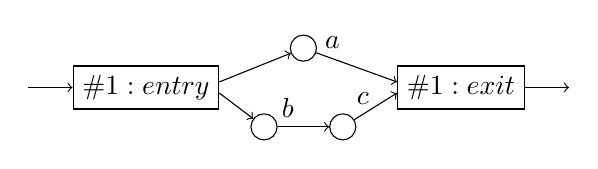
\begin{tikzpicture}
        \node[draw] (entry) at (-0.5, 0) {$\#1:entry$};
        \node[draw, circle] (up_a) at (1.5, 0.5) {};
        \node[draw, circle] (dw_b) at (1, -0.5) {};
        \node[draw, circle] (dw_c) at (2, -0.5) {};
        \node[draw] (exit) at (3.5, 0) {$\#1:exit$};

        \draw[->] ([xshift=-16]entry.west) -- (entry);
        \draw[->] ([yshift= 2pt]entry.east) -- (up_a);
        \draw[->] ([yshift=-2pt]entry.east) -- (dw_b);
        \draw[->] (dw_b) -- node[pos=0.2, above] (b) {$b$} (dw_c);
        \draw[->] (up_a) -- node[pos=0.2, above] (a) {$a$} ([yshift= 2pt]exit.west);
        \draw[->] (dw_c) -- node[pos=0.2, above] (c) {$c$} ([yshift=-2pt]exit.west);
        \draw[->] (exit) -- ([xshift=16]exit.east);
    \end{tikzpicture} \\ \vspace{0.3ex}
    \textit{NFA construction for $(a|bc)$}
\end{center}